% !TeX encoding = UTF-8
% !TeX spellcheck = fr_FR
% !TeX root = ../mythesis.tex
% !TeX program = pdflatex (build)
%%% TeXmaker : no 'magic comments' but set Root with Options > Set as master file

%useful stuff for what follows

\newcommand{\hf}{\hat{f}}
\newcommand{\hX}{\hat{X}}
\newcommand{\hY}{\hat{Y}}

\graphicspath{{./}{./fig/}{./chap_correlation/fig/}}

\chapter{Bogoliubov modes correlations in a polariton quantum fluid}

\label{chap:correlation}

The study of collective excitations in quantum fluids is fundamental to understand nonequilibrium dynamics and many-body interactions. Furthermore, the analog Hawking radiation
on which this work is focused, is expected to create non classical correlations between Bogoliubov modes, the event horizon acting as a two mode squeezer \cite{agullo_symplectic_2022}. The simplest manifestation
of paired correlated emission can be observed in the density fluctuations second order correlation function \cite{nguyen_acoustic_2015, carusotto_stimulatedfluid_2016,jacquet_quantum_2023,steinhauer_observation_2016}.
This observable exhibits a correlation pattern in the density fluctuations of the fluid on both side of the horizon.
Yet, this has been done only numerically in polaritonic system since the experiment would require to resolve the polariton lifetime $\sim 10 \mathrm{ps}$. However 
the strong photonic component of this system suggests that correlations between collective excitations modes must have an optical signature that could be addressed
with all the tools developed in quantum optics.
In this work, we report the first experimental measurement of correlations between collective excitation modes—Bogoliubov modes—in a static and homogeneous quantum fluid of microcavity exciton-polaritons.
 By using a balanced detection set-up, we measure intensity correlation between the normal and ghost branches, probing the fluctuation dynamics of the polariton fluid and extracting the spectral correlations of Bogoliubov excitations.
  We observe a clear enhancement of the intensity correlations when the polariton fluid operates near the turning point of the bistabilty due to the emergence of correlated phonon-like excitations. These correlations, seeded by quantum and thermal fluctuations, provide insights into the role of the nonlinear and phononic interactions in the collective excitations of a polariton quantum fluid.
This work paves the way towards the measurement of quantum correlations between modes emitted by an analog horizon.

\section{Quantum noise of an electromagnetic field}
\label{sec:intro_cv}
\subsection{Standard quantum limit}
Let us first consider a mode of the electromagnetic field with a frequency $\omega$, quantized within a box of volume V. At a fixed point in space, the electric field can be expressed using the photon creation and annihilation operators :

\begin{equation}
    \label{eq:field}
    \begin{aligned}
    \hat{E}(t) &= E_0\left( \hat{a} e^{-i\omega t} + \hat{a}^{\dagger} e^{i\omega t} \right) \\
    &= E_0\left(\hX\cos (\omega t) + \hY\sin(\omega t)\right)
    \end{aligned}
\end{equation}
where we introduced the quadrature operators $\hX$ and $\hY$ defined as :

\begin{equation}
    \label{eq:quad}
        \hX = (\hat{a} + \hat{a}^{\dagger})  \ \ \mathrm{and}  \ \
        \hY = i(\hat{a}^{\dagger} - \hat{a}).
\end{equation}
The amplitude of the field $E_0=\sqrt{\frac{\hbar \omega}{2\epsilon_0 V}}$ where $\epsilon_0$ is the vacuum permittivity, corresponds to the electric field of a single photon with energy $\hbar \omega$ in the quantization volume $V$. 
For a classical field, $X$ and $Y$ are real numbers and correspond to the real and imaginary parts of the complex field amplitude in the Fresnel representation as visible in \autoref{fig:fresnel} \textbf{a)}. In quantum mechanics,
the quadrature operators are conjugate variables. Indeed, by using the commutation relation of the photon creation and annihilation operators $[\hat{a},\hat{a}^{\dagger}]=1$, we obtain :

\begin{figure}
    \centering
    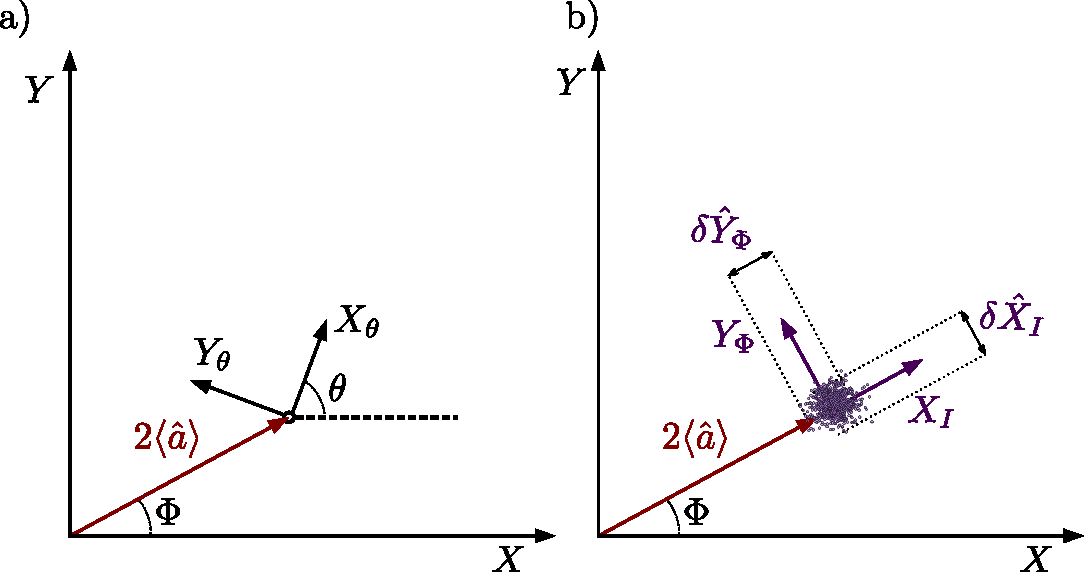
\includegraphics[width=0.8\textwidth]{chap_correlation/fig/fresnel.pdf}
    \caption{ \textbf{a)} Fresnel representation of a classical state. \textbf{b)} Quantum representation 
    of the quadrature operators. The cloud of points around the mean value $(\langle \hX \rangle, \langle \hY \rangle)$ represents several measurements of the same quantum state. The area of the cloud 
    is bounded from below by the Heisenberg uncertainty principle. The quadratures $\hX_{I}$ and $\hY_{\Phi}$ are the amplitude and phase quadratures respectively.}
    \label{fig:fresnel}
\end{figure}


\begin{equation}
    \label{eq:commut}
    [\hX,\hY] = 2i.
\end{equation}
Consequently, the quadrature operators are non-commuting variables and cannot be simultaneously measured with arbitrary precision. This is a direct consequence of the Heisenberg uncertainty principle stating that the product of the uncertainties in the two quadrature measurements is bounded from below by a constant value.
More precisely, the variances $\Delta X^2 = \langle \hX^2 \rangle - \langle \hX \rangle^2$ and $\Delta Y^2 = \langle \hY^2 \rangle - \langle \hY \rangle^2$ must satisfy the inequality :
\begin{equation}
    \label{eq:uncertainty}
    \Delta X^2 \Delta Y^2 \geq 1
\end{equation}
In contrast with the classical case, the vector $(\langle \hX \rangle, \langle \hY \rangle)$ representing the expectation values of the operators is associated with uncertainties whose area is bounded by the Heisenberg principle. 
The state most closely resembling a classical field is the one in which the fluctuations in both quadratures saturate \autoref{eq:uncertainty}. In this case, the uncertainty area assumes a circular shape with a diameter $E_0$ in the phase space, as illustrated in \autoref{fig:fresnel} \textbf{b)}. In this figure, the field and its fluctuations are not represented on the same scale; a laser field comprises a very large number of photons, whereas the fluctuations are much smaller. 
Such a minimum uncertainty state is referred to as a coherent state while the corresponding fluctuations define the standard quantum fluctuations. Coherent
states are typically produced by a laser way above threshold and are the eigenvectors of the annihilation operator $\hat{a}$.

\subsection{Intensity and phase fluctuations}

The choice of a given set of quadrature operators is arbitrary and corresponds to a choice of phase reference.
Moving to another set of operators $\hX_{\theta},\hY_{\theta}$ consists in a rotation in the phase space :

\begin{equation}
    \hX_{\theta} = \hX \cos(\theta) + \hY \sin(\theta) \ \ \mathrm{and} \ \
    \hY_{\theta} = -\hX \sin(\theta) + \hY \cos(\theta).
\end{equation}

The rotated operators satisfy the same commutation relation \ref{eq:commut} and the uncertainty relation \ref{eq:uncertainty} remains valid. 
However, a particular choice of quadratures is often made in the context of quantum optics \cite{grynberg_aspect_fabre} which consists in
choosing $\theta=\Phi$ where $\Phi$ is the phase of the mean field $\langle \hat{a}\rangle= |\hat{a}|e^{i\Phi}$.  The fluctuations of the corresponding quadrature
operators that we call $\hX_{I}$ and $\hY_{\Phi}$ are then proportional to intensity and phase fluctuations respectively as shown in \autoref{fig:fresnel} ~\textbf{b)}. In the case of 
a laser beam, the standard quantum limit is also referred to as the shot noise limit and corresponds to a poissonian statistics in the photon arrival time \cite{grynberg_aspect_fabre}.
Indeed, the measurement of the intensity of a laser beam is subject to statistical noise scaling as the square root of the mean number of photons in the beam.

\begin{equation}
    \label{eq:shotnoise}
    \Delta \hat{N}^2 = \langle \hat{N}\rangle
\end{equation}
From an experimental point of view, this relation is helpful since it provides a direct way to infer the standard quantum limit from an intensity measurement.   


\subsection{Squeezed states}
While vacuum fluctuations serve as a reference for quantum fluctuations, there is nevertheless no fundamental restriction against obtaining states in which the fluctuations of a given quadrature, $\hX_{\theta}$, are reduced below the standard quantum limit. Indeed, the Heisenberg inequality pertains to the product of uncertainties.
 This inequality remains satisfied provided that the fluctuations in the orthogonal quadrature $\hY_{\theta}$ increase accordingly. Graphically, their representation is obtained by squeezing the uncertainty area along the direction of the quadrature $\hX_{\theta}$ and stretching it along the direction of $\hY_{\theta}$. A typical representation of such a state in the phase space is shown in \autoref{fig:squeezed_state}. The resulting states are referred to as a squeezed state, and are of great interest 
 in quantum optics as they can be used to enhance the sensitivity of measurements. As an example, phase squeezed state are used in LIGO-VIRGO infrastructures to resolve the infinitesimal displacements of the interferometer mirrors induced by the gravitational waves.

\begin{figure}
    \centering
    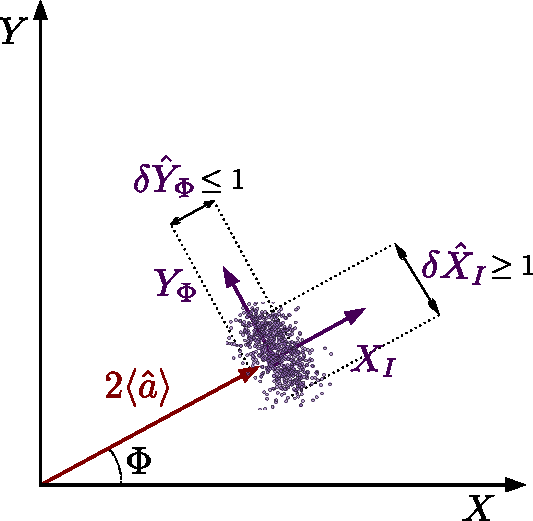
\includegraphics[width=0.5\textwidth]{chap_correlation/fig/fresnel_squeezed.pdf}
    \caption{Representation of a squeezed state in the phase space. The uncertainty area is squeezed below the SQL along the $\hY_{\Phi}$ phase quadrature and correspondingly stretched along the $\hX_{I}$ intensity quadrature. The uncertainty area is still bounded by the Heisenberg uncertainty principle.}
    \label{fig:squeezed_state}
\end{figure}



\section{Photodectection}
\label{sec:photodetection}


A photodetector is a device that converts the energy of a photon into an electrical signal. The most common type of photodetector is the photodiode, which operates by generating a current in response to the absorption of photons. 
In principle, such devices allows to acquire and process all the information contained in the electromagnetic field by electronic means.
However, an optical field oscillates at hundreds of terahertz, which is far beyond the bandwidth of any electronic device. A photodiode can thus 
only provide a time-averaged signal, which is proportional to the intensity of the field. More precisely, the mean value of the photo-current $\bar{i}$ is proportionnal to the incoming photon flux as :

\begin{equation}
    \label{eq:photocurrent}
    \bar{i} = \eta e \dfrac{P}{\hbar\omega}
\end{equation}
where $\eta$ is the quantum efficiency of the photodetector, $e$ is the electron charge, $P$ is the power of the incoming light and $\hbar\omega$ is the energy of a single photon. 
In the ideal case $\eta=1$ where $100\%$ of the photons are converted into electrons the current statistics reproduce exactly the statistics of the incoming light.
However, in practice, the quantum efficiency is always less than one and the photodetector introduces losses that add to the photonic losses that the incoming beam may has already undergone.
Such losses are random events and subsequently lead any statistics to become Poissonian when they are large enough.


This being said, a incoming photon flux shot noise limited will produce a photocurrent that also follows a Poissonian statistics. For a mean number 
of electron $N_e$ produced by the photodetector, the variance is :

\begin{equation}
    \label{eq:n_e_variance}
    \Delta N_e^2 = N_e.
\end{equation}
From which we deduce the variance of the photocurrent on a time interval $\Delta t$ :
\begin{equation}
    \label{eq:photocurrent_variance}
    \Delta i^2 = \dfrac{e^2\Delta N_e^2}{\Delta t^2}=\dfrac{e^2N_e}{\Delta t^2}.
\end{equation}
Furthermore, by writting $N_e=\bar{i}\Delta t/e$ we obtain :
\begin{equation}
    \label{eq:photocurrent_variance2}
    \Delta i^2 = \dfrac{e\bar{i}}{\Delta t}.
\end{equation}
This relation shows that the variance of the photocurrent is inversely proportional to the time interval over which the current is measured. In the frequency
domain it means that the variance is proportional to the bandwidth of the measurement apparatus $\delta f=1/2\Delta t$. 
Furthermore, in the case where the measurement devices can be modeled by a narrow band-pass filter centered on an analysis frequency $\omega_c$ it can be shown \cite{fabre_houches_97}
that the variance of the photocurrent is related to its power spectral density (PSD) as :

\begin{equation}
    \label{eq:photocurrent_variance3}
    \Delta i^2 = 2\delta f S_i(\omega).
\end{equation}
This is precisely how a spectrum analyzer works. It measures the power spectral density of the photocurrent $S_i(\omega)$ by integrating its variance over a given bandwidth $\delta f$ usually limited by the resolution 
bandwidth (RBW) of the spectrum analyzer.
At the end, we have a way to measure the power spectral density of the incoming light field by measuring the variance of the photocurrent. 
Let us now see how such a device can be used to measure the correlations between two fields.

\section{Balanced detection}
Intensity balanced detection is a common detection scheme used to suppress the classical noise commonly present in optical measurements and measure the intensity noise of a beam.
The basic principle of this technique is to use two photodetectors, each measuring the intensity of an optical field, and to subtract their output photo-currents. If the two 
beams share the same classical noise, the subtraction will cancel it out, leaving only the quantum correlations. A representation of the balanced detection scheme is shown in \autoref{fig:balanced_detection}.
Such apparatuses are typically also capable of measuring the sum of the two photocurrents, whose noise is proportional to the total noise of the two beams.
 However,
as we will see in the next section, measuring the difference together with the individual photo-currents is sufficient to obtain the correlation function of the two fields.
\begin{figure}
    \centering
    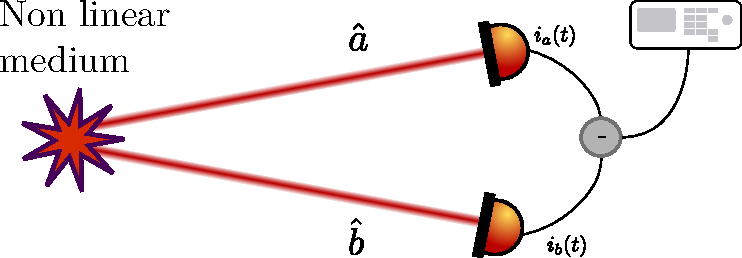
\includegraphics[width=0.8\textwidth]{chap_correlation/fig/balanced_detection.pdf}
    \caption{Balanced detection scheme. Example of a typical nonlinear medium producing two modes of the electromagnetic field $\hat{a}$ and $\hat{b}$. Each of them is sent to a photodiode that produces a photo-current carrying the noise
    of the beams. The output photo-currents are then subtracted to cancel the classical noise and sent into a spectrum analyzer.}
    \label{fig:balanced_detection}
\end{figure} 

\subsection{Difference measurement}
Let us consider two fields $\hat{a}$ and $\hat{b}$ impinging on two photodetectors as shown in \autoref{fig:balanced_detection}. Their respective intensities 
are given by their number operator $\hat{N}_a=\hat{a}^\dagger\hat{a}$ and $\hat{N}_b=\hat{b}^\dagger\hat{b}$.
We are interested in the intensity difference operator $\hat{N}_-$ defined as :
\begin{equation}
    \label{eq:diff_op}
    \hat{N_-} = \hat{a}^\dagger\hat{a} - \hat{b}^\dagger\hat{b}.
\end{equation}

As explained above, it is convenient to linearize each operator around its mean value :
\begin{equation}
    \begin{aligned}
    \hat{a} &= |\alpha|e^{i\Phi} + \delta \hat{a} \\
    \hat{b} &= |\beta|e^{i\Psi} + \delta \hat{b}
    \end{aligned}
\end{equation}
where $|\alpha|e^{i\Phi}$ and $|\beta|e^{i\Psi}$ are the mean values of the two fields and $\delta \hat{a}$ and $\delta \hat{b}$ are their respective fluctuations.
The difference operator can then be expressed to first order in the fluctuations as :
\begin{equation}
    \label{eq:diff_op2}
    \begin{aligned}
    \hat{N_-} &= (|\alpha|e^{-i\Phi}+\delta \hat{a}^\dagger)(|\alpha|e^{i\Phi}+\delta \hat{a}) - (|\beta|e^{-i\Psi}+\delta \hat{b}^\dagger)(|\beta|e^{i\Psi}+\delta \hat{b}) \\
    &= |\alpha|^2 - |\beta|^2 +(|\alpha|\delta \hX_a^\Phi - |\beta|\delta \hX_b^\Psi) 
    \end{aligned}
\end{equation}
The mean value $<N_->=|\alpha|^2-|\beta|^2$ provides information about the average intensity difference between the two beams. In the balanced case—that is, when this difference vanishes—the fluctuations of the difference can be expressed as:
\begin{equation}
    \label{eq:diff_fluctuation}
    \delta \hat{N_-} = |\alpha|(\delta \hX_a^\Phi - \delta \hX_b^\Psi).
\end{equation}
If the two fields are intensity correlated, the fluctuations of the difference operator is reduced. The case where $<N_->\neq0$ requires a more detailed analysis. In particular, it should be noted that in this situation, the individual quantum noise of each mode plays a role in the measurement of correlations. For further discussion, one can refer to \cite{treps_fabre_criteria_2004}. 
In practice, we will measure the variance of the difference operator as we will see in the next section.
\section{Correlations in continuous-variables quantum optics}

\label{sec:corr_cv}
As a very general statement, two quantities are usually correlated if they ultimately originate from the same source or quantum process. In this case, a knowledge of one of the two quantities gives information about the other.
Take the example of a two photons emission by a non linear process such as a Type II spontaneous parametric down conversion (SPDC). Their correlations is of several natures. The first and most obvious one is temporal in the sense that the two photons are emitted at the same time. This can be
quantified by looking at the second order intensity correlation function $g^{(2)}(t,t')$, which is the probability of detecting a photon at time $t$ and another one at time $t'$ \cite{hanbury_brown_twiss_1956}. They can also 
be correlated through their polarization meaning that if one photon is detected in a given polarization, the other one will be detected in the orthogonal polarization. Reversing the picture,
the measurement of a given type of correlations can thus provide information about the quantum nature of the process that generated them.

\subsection{Correlation function.} Let us consider a quantum operator evolving in time $\hat{f}(t)$. The autocorrelation of $\hf$ at time $t$ and $t'$ is defined as :


\begin{equation}
    \label{eq:autocorr}
    C_{\hf}(t,t') = \langle \hf(t)\hf(t') \rangle = \langle \delta \hf(t) \delta \hf(t') \rangle
\end{equation}
where $\delta \hf(t) = \hf(t) - \langle \hf(t) \rangle$ is the fluctuation of the operator around its expectation value. If the process at stake 
is stationary, $\langle \hf(t) \rangle$ does not depend on $t$ and the correlation function depends only on the time difference $\tau= t-t'$ \cite{bachor_guide_1998}. In this case,
the Wiener-Khinchin theorem states that the autocorrelation function is related to the spectral density of the field $\mathcal{S}_{\hf}(\omega)$ by a Fourier transform \cite{fabre_houches_97} :

\begin{equation}
    \label{eq:autocorr_spectral}
    S_{\hf}(\omega) = \int_{-\infty}^{+\infty} C_{\hf}(\tau) e^{-i\omega \tau} d\tau.
\end{equation}
In the same manner, it is possible to define the cross-correlation between two operators $\hf_a$ and $\hf_b$ as :

\begin{equation}
    \label{eq:crosscorr}
    C_{\hf_a,\hf_b}(t,t') = \langle \hf_a(t)\hf_b(t') \rangle = \langle \delta \hf_a(t) \delta \hf_b(t') \rangle
\end{equation}
The corresponding cross power spectral density (for stationary processes) is given by the Fourier transform of this correlation function :
\begin{equation}
    S_{ab}(\omega) = \int_{-\infty}^{+\infty} C_{ab}(\tau) e^{i \omega \tau} \, d\tau
\end{equation}
If we are now interested in the autocorrelation of the difference operator $\hat{N}_-$ defined in \autoref{eq:diff_op}, one can express the PSD of the difference operator as  \cite{bachor_guide_1998} :

\begin{equation}
    \label{eq:diff_psd}
    S_{-}(\omega) = S_{a}(\omega) + S_{b}(\omega) - 2S_{ab}(\omega).
\end{equation}
where $S_{a}(\omega)$ and $S_{b}(\omega)$ are the power spectral densities of the number operators $\hat{N}_a$ and $\hat{N}_b$ respectively.
From this, we define the normalized cross-correlation function between the two operators as :
\begin{equation}
    \label{eq:crosscorr_norm}
    C_{ab}(\omega) = \dfrac{S_{ab}(\omega)}{\sqrt{S_a(\omega) S_b(\omega)}}.
\end{equation}
The PSD of the difference operator can then be expressed in terms of the normalized cross-correlation function as :
\begin{equation}
    \label{eq:diff_psd2}
    S_{-}(\omega) = S_{a}(\omega) + S_{b}(\omega) - 2\sqrt{S_a(\omega) S_b(\omega)}C_{ab}(\omega).
\end{equation}
Due to the Cauchy-Schwarz inequality, $C_{ab}$ is bounded between $-1$ and $1$. A value of $C_{ab}(\omega)=1$ indicates that the two operators are perfectly correlated, while $C_{ab}(\omega)=-1$ indicates that they are perfectly anti-correlated. 

\bigskip

Finally, if we invert \autoref{eq:diff_psd2}, we can express the normalized cross-correlation in terms of the PSDs as :
\begin{equation}
    \label{eq:crosscorr_norm2}
    C_{ab}(\omega) = \dfrac{S_{-}(\omega) - S_a(\omega) - S_b(\omega)}{-2\sqrt{S_a(\omega) S_b(\omega)}}.
\end{equation}
By measuring the PSD of the difference operator $S_{-}(\omega)$ and the individual PSDs $S_a(\omega)$ and $S_b(\omega)$, we can thus obtain the normalized cross-correlation function $C_{ab}(\omega)$ between the two operators.

\subsection{Bogoliubov modes correlations}

Let us now consider a static homogeneous polariton fluid created by a pump with frequency and wavevector $(\omega_p$, $k_p$), operating on the high density branch of the bistability curve as we did in the previous chapters.
We set our description in the rotating frame of the pump laser so that in the following we will drop the pump frequency $\omega_p$ and wavevector $k_p$.
A given Bogoliubov mode at $(k,\omega)$ on the normal branch, and its conjugate mode at $(-k,-\omega)$ on the ghost branch, are expected to be correlated.
Indeed, they ultimately result from a four-wave mixing process that is the parametric scattering of two pump polaritons into two Bogoliubov modes at $(k,\omega)$ and $(-k,-\omega)$.
More precisely, the phase matching and energy conservation conditions of the four-wave mixing process read as :

\begin{equation}
    (0,0)+(0,0) \rightarrow (k,\omega)+( -k,-\omega).
\end{equation}

\textbf{Bogoliubov coefficients.} According to the Bogoliubov theory, the Bogoliubov amplitudes $u_{k}$ and $v_{k}$ related to the normal branch mode and the ghost branch mode respectively are given by \cite{castin_bose-einstein_2001,pitaevskij_bose-einstein_2016} :

\begin{align}
    u_k &= \sqrt{\frac{1}{2} \left( \frac{\epsilon_k + 2g n_0-\delta}{\omega^+_B(k)} + 1 \right)}, \\
    v_k &= -\sqrt{\frac{1}{2} \left( \frac{\epsilon_k + 2g n_0-\delta}{\omega^+_B(k)} - 1 \right)}.
\end{align}
where $gn_0$ is the interaction energy, $\epsilon_k=\hbar k^2/2\mlp$ is the kinetic energy with $\mlp$ the polaritons effective mass, and $\omega^+_B(k)$ is the positive norm Bogoliubov frequency :

\begin{equation}
    \omega^{+}_B(k)=\sqrt{\left(\dfrac{\hbar k^2}{2\mlp}-\delta +2g n_0\right)^2 - \left(g n_0\right)^2}
\end{equation}
with $\delta = \omega_p - \omega_{LP}$ the detuning between the pump laser and the polariton resonance frequency $\omega_{LP}$ at zero wavevector. Note that 
the reservoir contribution was not taken into account without loss of generality since its contribution can be included in the detuning $\delta$.

\bigskip

\textbf{Stimulated emission.} The Bogoliubov modes can be probed by injecting a weak probe laser beam at a specific wavevector $k_{\mathrm{pr}}$ and frequency $\omega_{\mathrm{pr}}$, chosen to be resonant with the mode at $(k_{\mathrm{pr}}, \omega_{\mathrm{pr}})$ on the normal branch, as in previous experiments. 

As explained in \autoref{chap:generation_transonic_fluid}, this results in the stimulation of a four-wave mixing process, leading to the emission of two optical beams at $(k_{\mathrm{pr}}, \omega_{\mathrm{pr}})$ and $(-k_{\mathrm{pr}}, -\omega_{\mathrm{pr}})$. 
Using the input-output formalism~\cite{I_frerot_PRX_2023}, one can compute the expected intensities of the emitted beams on the normal and ghost branches as:


\begin{equation}
    \label{eq:uv_intensity2}
    \begin{aligned}
    I_N(k_{pr},\omega_{pr}) &= |u_{k_{pr}}|^4 |\alpha|^2  \  \mathrm{for \ the \ normal \ branch } \\
    I_G(-k_{pr},-\omega_{pr}) &= |v_{k_{pr}}u_{k_{pr}}|^2 |\alpha|^2 \ \mathrm{ for \ the \ ghost \  branch.}
    \end{aligned}
\end{equation}
where $|\alpha|^2$ is the intracavity probe intensity. This two intensities are expected to yield high correlation since they result from a nonlinear four-wave mixing process \cite{glorieux_quantum_2011,romanelli_4wm_2007}. Measuring this correlation is the goal of this experiment.

By computing the ratio of the two intensities, we can eliminate the probe contribution and obtain the Bogoliubov coefficients ratio $u_{k_{pr}}^2/v_{k_{pr}}^2$. 
The asymptotic behavior of this ratio is then expected to scale as~\cite{castin_bose-einstein_2001}. :

\begin{equation}
    \begin{aligned}
    \dfrac{u_{k_{pr}}^2}{v_{k_{pr}}^2} & \sim \dfrac{\hbar^2k^4}{\mlp^2g^2n_0^2} \  \ \ &\mathrm{when} \ k_{pr} \to +\infty \\
    &\sim 1 \ \ &\mathrm{ when} \ k_{pr} \to 0.
    \end{aligned}
\end{equation}
As a result, the beams on the normal and ghost branches are balanced at low wavevectors, which is expected to enhance the correlations between the two beams, as will be discussed in the following section.


\section{Experimental implementation}
\label{sec:exp_impl}

The set up used is similar to the one used in the previous experiment with the addition of a balanced detection scheme that will be detailled in the next section. 
The microcavity is the same as the one used in the previous chapters but the experiment is run at the working point B10-C10 (see \autoref{fig:sample_map}).

\bigskip

\subsection{Bogoliubov coefficients measurement}


We create a static polariton fluid by shinning a pump laser beam of diameter $w=\SI{100}{\micro\meter}$ at normal incidence on the microcavity ie at $k_p=0$. The laser is detuned from the polariton resonance by
$\delta = \SI{35}{\giga\hertz}$ in order to operate in a bistable regime. The pump laser is $\sigma_+$ polarized in order to excite a single polariton population \cite{timofeev_exciton_2012}. A typical real space image of the polariton fluid is shown in \autoref{fig:real_space} \textbf{a)}. 


\begin{figure}
    \centering
    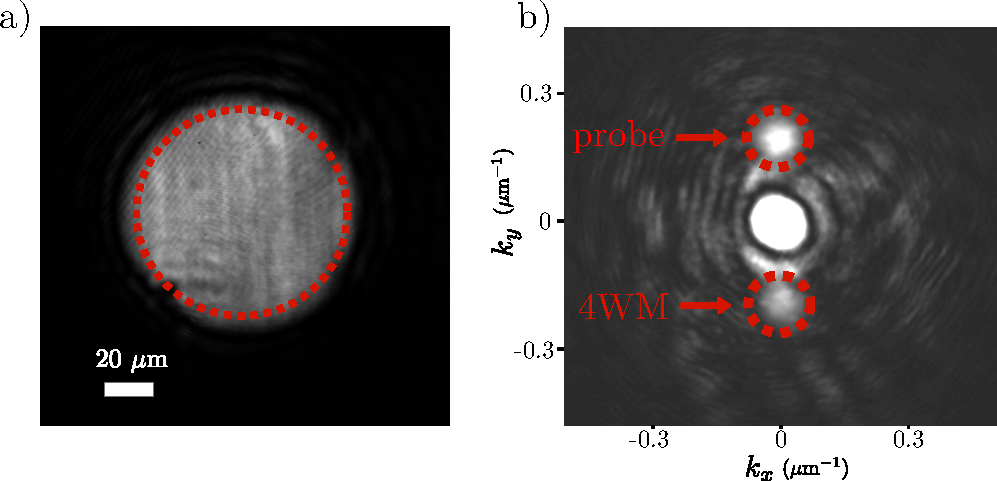
\includegraphics[width=1\textwidth]{chap_correlation/fig/r_and_k_space.pdf}
    \caption{\textbf{a)} Real space image of a polariton fluid operating on the high density branch of the bistability loop. The image is taken at the working point B10-C10. The red dashed circle represents
    the pinhole applied to the image to filter out the signal coming from the edges of the fluid. \textbf{b)} Corresponding k-space image of the polariton fluid when a weak probe is exciting the normal branch at $k_{pr}=\SI{0.2}{\per\micro\meter}$. 
    The direct transmission of the probe is pointed out by the red arrow on top of the image while its four wave mixing signal is visible at $-k_{pr}$. The red dasehd circles represent the pinholes applied 
    in the fourier plane to isolate each signal before sending it to the balanced detection scheme. }
    \label{fig:real_space}
\end{figure}


\bigskip

To begin with, the collective excitation spectrum of the fluid is measured with the same method as in \autoref{chap:generation_transonic_fluid}. The pump laser intensity is set to operate close to the turning point of the higher branch of the bistability loop but sufficiently far from it to have a stable polariton fluid. 
The normal branch shown in \autoref{fig:uv_analysis} \textbf{a)} is measured through direct excitation ie by placing pinholes that track the probe wavevector in the Fourier space at each energy scan.
 Conversely, the ghost branch shown in \textbf{b)} is measured through 4WM excitation meaning that the pinholes are systematically positioned at the opposite wavevector $-k_{pr}$. At each couple $(k,\omega)$ and $(-k, -\omega)$ the corresponding intensities are measured by fitting the resonance peaks 
by a Lorentzian function. As outlined by the previous section, by then computing the ratio of the two quantities, the probe contribution disappears and we can have acces to the Bogoliubov coefficients ratio $u_{k_{pr}}^2/v_{k_{pr}}^2$. 
\autoref{fig:uv_analysis} \textbf{c)} shows this ratio as a function of the probe wavevector $k_{pr}$. At low wavevector, the ratio tends to a constant value which is expected from the Bogoliubov theory as explained in the previous section. A quantitative estimate of this value cannot be extracted from the data, as the measurement method does not allow for discrimination between the two conjugate modes at low wavevectors.
However, one can estimate that the ratio is close to one which is consistent with the theoretical prediction.
At high wavevector $u_{k_{pr}}^2/v_{k_{pr}}^2$ is expected to follow a $k^4$ law as previously explained. To discuss this feature, we take the data for $|k_{pr}| > 1/\xi\approx\SI{0.35}{\per\micro\meter}$ and fit them with a power law of the form $ak^\beta$ with $a$ and $\beta$ as fitting parameter. The healing length $\xi=\SI{3}{\micro\meter}$ is estimated from the detuning $\delta =\SI{35}{\giga\hertz}$ which is slightly lower than the interaction energy $gn_0$ since the system operates close to the turning point of the bistability loop.

\bigskip

The resulting fits are represented by the red dashed lines in \autoref{fig:uv_analysis} \textbf{c)}. The fit gives a value of $\beta=3.74\pm0.5$ for negative wavevector whereas for positive wavevector we obtain $\beta=1.47\pm{0.5}$. The first value is consistent with the Bogoliubov theory prediction of $\beta=4$ while the second one is not. The uncertainty on $\beta$ is of $13\%$ for $k<0$ and $34\%$ for $k>0$. 
 This asymmetry between the two branches is not well understood and may be due to a sample effect that is not perfectly isotropic. Indeed, 
as explained in \autoref{chap:generation_transonic_fluid}, the sample exhibits a wedge which is a small tilt of the microcavity DBR mirrors. This creates a direction along which the photon resonance energy increases as a function of the cavity width.
This breaking of symmetry may result in a $k$-dependent efficiency of the emission that is not taken into account in the initial model. A way to verify this hypothesis would be to precisely characterize the wedge as well as the $k$-dependance of the DBR reflectivity and run numerical simulations of angle and energy resolved emission. 

It is worth noticing that at low wavevector $|k_{pr}|<\SI{0.5}{\per\micro\meter}$ where $k$ and $-k$ are closer to each other, symmetry between the branch is restored which support the anisotropy hypothesis 
we just made.

\bigskip

\textbf{Bogoliubov coefficients.} The Bogoliubov coefficients $u_{k_{pr}}$ and $v_{k_{pr}}$ can be separately extracted from the ratio $u^2/v^2$ by using the normalization condition $u^2-v^2=1$. The 
results are shown in \autoref{fig:uv_analysis} \textbf{d)}. While we observe a clear enhancement of both coefficients at low wavevector, we do not observe the $1/k$ divergence expected from the Bogoliubov theory. This is not due to the incapacity of the experimental method to disitinguish  between the normal and the ghost the modes a low wavevector. Indeed,
such a divergence should be observed in the overall intensity collected by the pinhole.
In fact, in the litterature \cite{pitaevskij_bose-einstein_2016,castin_bose-einstein_2001,pethick_bose-einstein_2008}, the $1/k$ behavior is computed for a homogeneous and infinite condensate. In practice, eventhough the polariton fluid is homogeneous it has a finite size of $w=\SI{100}{\micro\meter}$. The latter,
limits the minimum wavevector that can be probed to $k_{min}=\pi/w\approx\SI{0.03}{\per\micro\meter}$. In other words, it is not possible to excite modes that correspond to interactions ranges greater than the size of the fluid.

In view of measuring correlations between the Bogoliubov modes, the validation that the emissions in the two branches become balanced at low wavevector suggests that correlations should increase in this regime \cite{treps_fabre_criteria_2004}. This is precisely what we observe as we will see in the next section.


\begin{figure}
    \centering
    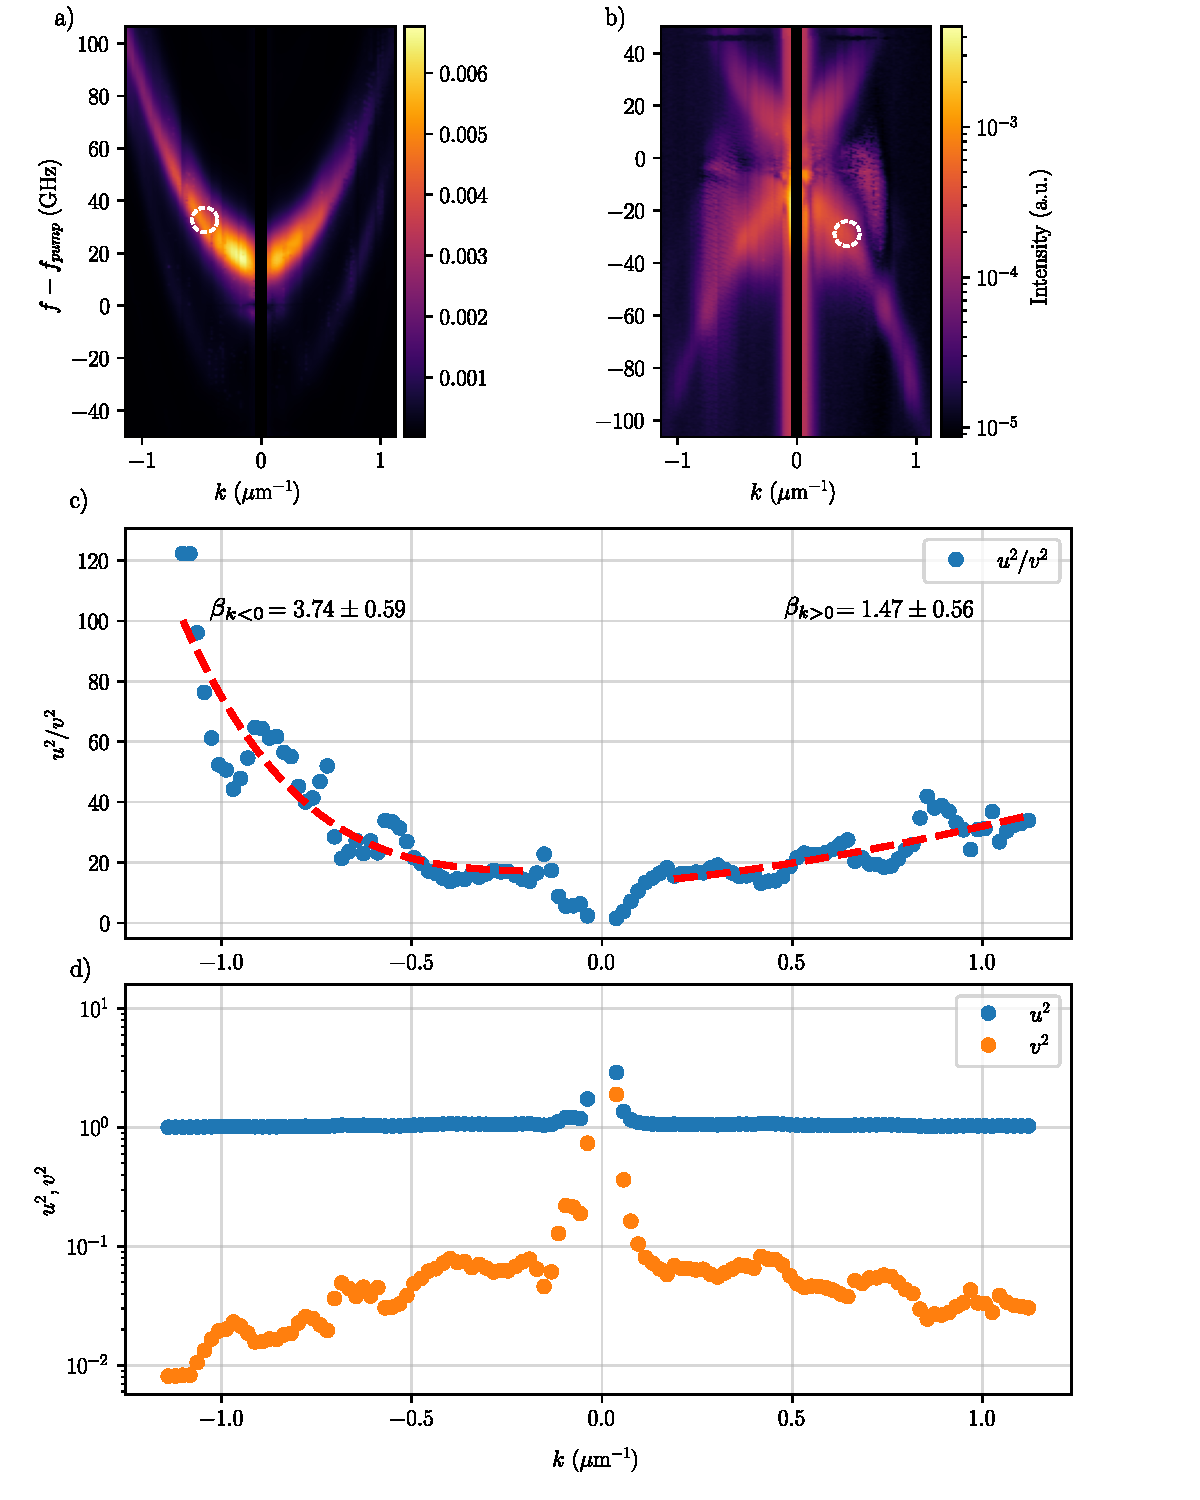
\includegraphics[width=1\textwidth]{chap_correlation/fig/uv_analysis.pdf}
    \caption{\textbf{Bogoliubov dispersion measurement.} \textbf{a)} Normal branch measurement. \textbf{b)} Ghost branch measurement. As explained in \autoref{chap:generation_transonic_fluid}, the black solid rectangle
    centered at $k=0$ on both plots represents the region where the two conjugate modes start to overlap in the $k$-space and thus cannot be resolved. The white dashed circles represent two conjugated Bogoliubov modes whose emission are compared to extract the Bogoliubov coefficients $u$ and $v$.}
    \label{fig:uv_analysis}
\end{figure} 

\subsection{Bogoliubov modes correlations}
\label{sec:exp_corr}


\subsubsection{Shot noise calibration}
Since we are interested in measuring correlations produced by the non linear four wave mixing process, it is necessary to make sure that both the lasers
injected in the microcavity don't introduce any classical noise in the system. Indeed, as explained in \cite{treps_fabre_criteria_2004}, if the laser used to stimulate non linear effect carry classical noise, both of the emitted beam 
will be classically correlated which will result in a strong noise reduction in the difference photocurrent and artificially enhance the correlations.
To verify that the lasers are shot noise limited, we send one of them on a half wave plate followed by a polarizing beam splitter (PBS). This enables to precisely balance the two outputs of the PBS before sending them to the balanced detection scheme and make sure 
that any classical noise is cancelled out. Then, the intensity of the laser is ramped up. At each intensity value, the PSD is measured by a spectrum analyzer in order to determine the linear relation between 
the laser power and the intensity variance. Since all the classical noise has been removed, this variance reflects the poissonian statistics stemming from the intrinsic quantum noise of the lasers as explained in the previous section. As this statistic is universal,
there is no need to make the measurement for the two lasers and the linear coefficient relating intensity and noise is fixed by the measurement apparatus \cite{bachor_guide_1998}.

\begin{figure}
    \centering
    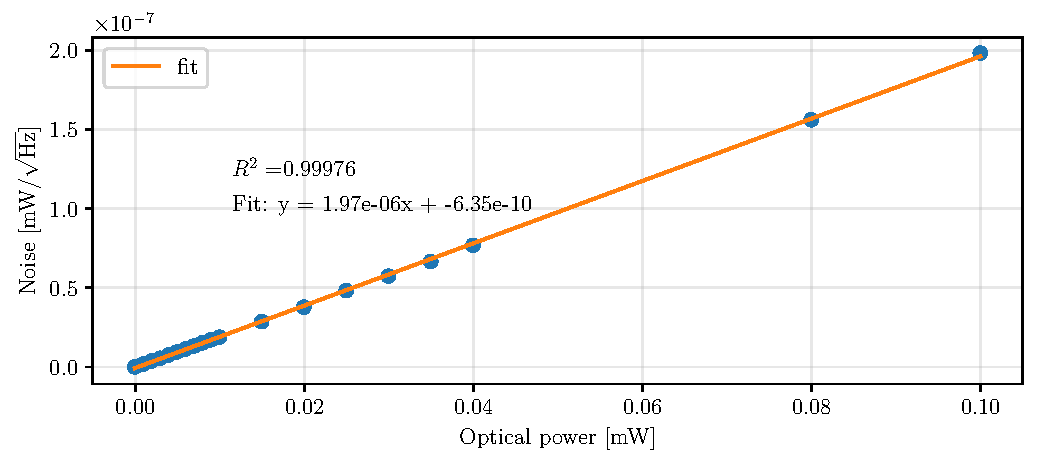
\includegraphics[width=1\textwidth]{chap_correlation/fig/noise_vs_optical_power.pdf}
    \caption{Shot noise calibration. The variance of the photocurrent is measured as a function of the laser power. The dark noise of the apparatus measurement has been substracted. The linear fit gives the coefficient relating the intentity of the laser and the shot noise level.}
    \label{fig:calibration}
\end{figure}

\bigskip

The results are presented in \autoref{fig:calibration}.
As expected, the variance of the photocurrent is linear with the laser power. This calibration curve is then used to make sure that the lasers are shot noise limited by verifying that, for a given laser power 
its power spectral density falls on the calibration curve. This verification was done for both lasers used in the experiment, the pump and the probe, and both of them were found to be at the standard quantum limit ensuring that no classical noise is 
 introduced in the system.

Of course, the settings of the spectrum analyzer as well as the photodetector must be exactly the same as the ones used for the calibration process. Since the quantum noise 
is a white noise, the calibration as well as the experiment can be in principle done at any frequency. However, it is convenient to chose an analysis frequency at least in the MHz range to the $1/f$ electronic noise as well as classical noises like vibrations while staying in the photodetector bandwidth of few MHz. These vibrations are mainly due to the vacuum pump connected to the cryostat whose 
frequency do not exceed hundreds of kilohertz. Further increasing the analysis frequency mean that the photodetector bandwidth must be accordingly increased which would result in a reduction of the apparatus gain and thus of the signal to noise ratio.
To have the best compromise between these constraints, the calibration and the experiment were done at $\SI{1.5}{\mega\hertz}$. 


 


The photodiodes used in this experiment are industrial Thorlabs PDB450A photodiodes with adjustable gain. The latter is set to $10^4$ in order to have a bandwidth of $\SI{4}{\mega\hertz}$.
The spectrum analyzer is a RIGOL DSA-815 in zero span mode at $\SI{1.5}{\mega\hertz}$. The resolution bandwidth (RBW) as well as the video bandwidth (VBW) are set to $\SI{100}{\kilo\hertz}$ in order to have a good compromise between the signal to noise ratio and the measurement time.
The sweep time is set to $\SI{100}{\milli\second}$.


\begin{figure}
    \centering
    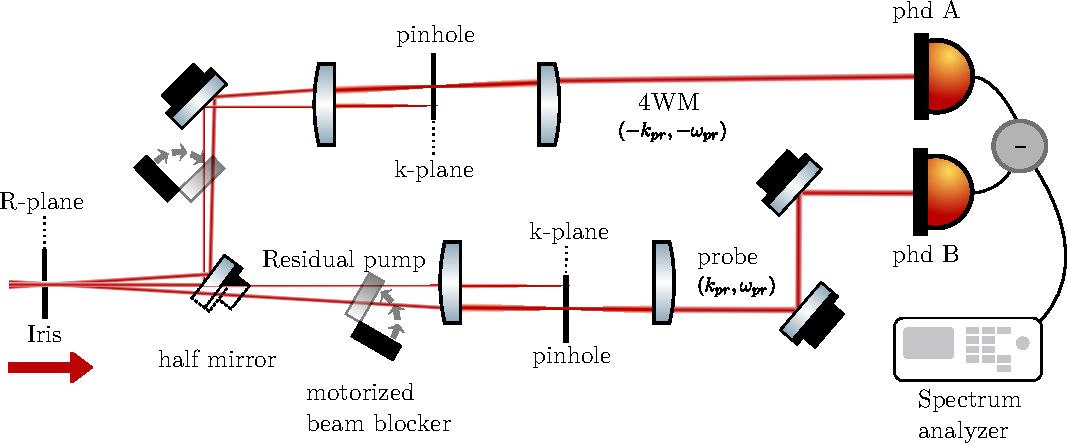
\includegraphics[width=1\textwidth]{chap_correlation/fig/half_mirror.pdf}
    \caption{Experimental set up used to measure the correlations between Bogoliubov modes. The red arrows represent the propagation direction of the light.
    The first real space filtering is done with an adjustable iris diaphragm while the filtering in Fourier space is done with pinholes of diameter $w=\SI{300}{\micro\meter}$ to match the size of the 
    probe. A motorized beam blocker is placed on each optical path to measure the noise of each beam separately. The focal lengths of the lenses are chosen to magnify the image so its matches the size of the photodiodes sensors that are $d=\SI{800}{\micro\meter}$ in diameter. The two photodiodes are connected to a spectrum analyzer in zero span mode at $\SI{1.5}{\mega\hertz}$. The resolution bandwidth (RBW) and the video bandwidth (VBW) are set to $\SI{100}{\kilo\hertz}$.}
    \label{fig:set_up_balanced}
\end{figure}

\subsubsection{Balanced detection}
Once the polariton fluid is established, we fix the probe wavevector to $k_{pr}=\SI{0.2}{\per\micro\meter}$ and tune the laser frequency to be resonant with the normal branch of the Bogoliubov dispersion. The field outgoing the microcavity is then directed to a balanced detection setup, illustrated in \autoref{fig:set_up_balanced}.
To measure the correlations between the Bogoliubov modes, it is essential to isolate the two conjugate modes from each other but also from the pump. 

\bigskip

\indent If the photodiodes collect residual light from the pump, the detection scheme may yield a spurious non-zero correlation even in the absence of the probe. Indeed, although the pump laser generating the mean field is shot-noise limited, the photonic component of the polariton fluid escaping the microcavity is not.
This excess noise originates from the Kerr effect inside the cavity, which leads to self-phase modulation of the polariton field. As a result, additional intensity and phase fluctuations are introduced in the fluid. If one spatially isolate two regions of the fluid, the fluctuations in the mean field will be correlated, leading to a non-zero correlation signal in the balanced detection scheme.
However, these correlations do not stem from the nonlinear scattering process under investigation, but rather from the single mode character of the polariton fluid as demonstrated in \cite{a_baas_quantum_degeneracy2006}.

\bigskip

\indent To prevent this, we first perform a spatial filtering of the polariton fluid in real space, as illustrated in \autoref{fig:set_up_balanced}. The real-space image of the polariton fluid is filtered using an adjustable iris, whose aperture is set to match the diameter of the pump beam.
The purpose of this filtering is to remove the light coming from the edges of the polariton fluid, which, as explained in the previous chapter, expels polaritons at high momentum and may yield a spurious signal in the detection scheme.
The filtered image is then left to propagate, allowing the Bogoliubov signals at $k_{\mathrm{pr}}$ and $-k_{\mathrm{pr}}$, as well as the mean field at $k = 0$, to become spatially separated in the far field.
 Then, a half mirror is used to split the light into two paths as shown in \autoref{fig:set_up_balanced}.
At this stage, both paths still contain mean field photons. To remove them, another filtering is applied in the Fourier plane to isolate the Bogoliubov modes as shown in \autoref{fig:real_space} \textbf{b)}. This picture shows the whole $k$-space image for the sake of clarity, but in practice,
the top and bottom halves belong to two different paths of the balanced detection scheme.


\begin{figure}
    \centering
    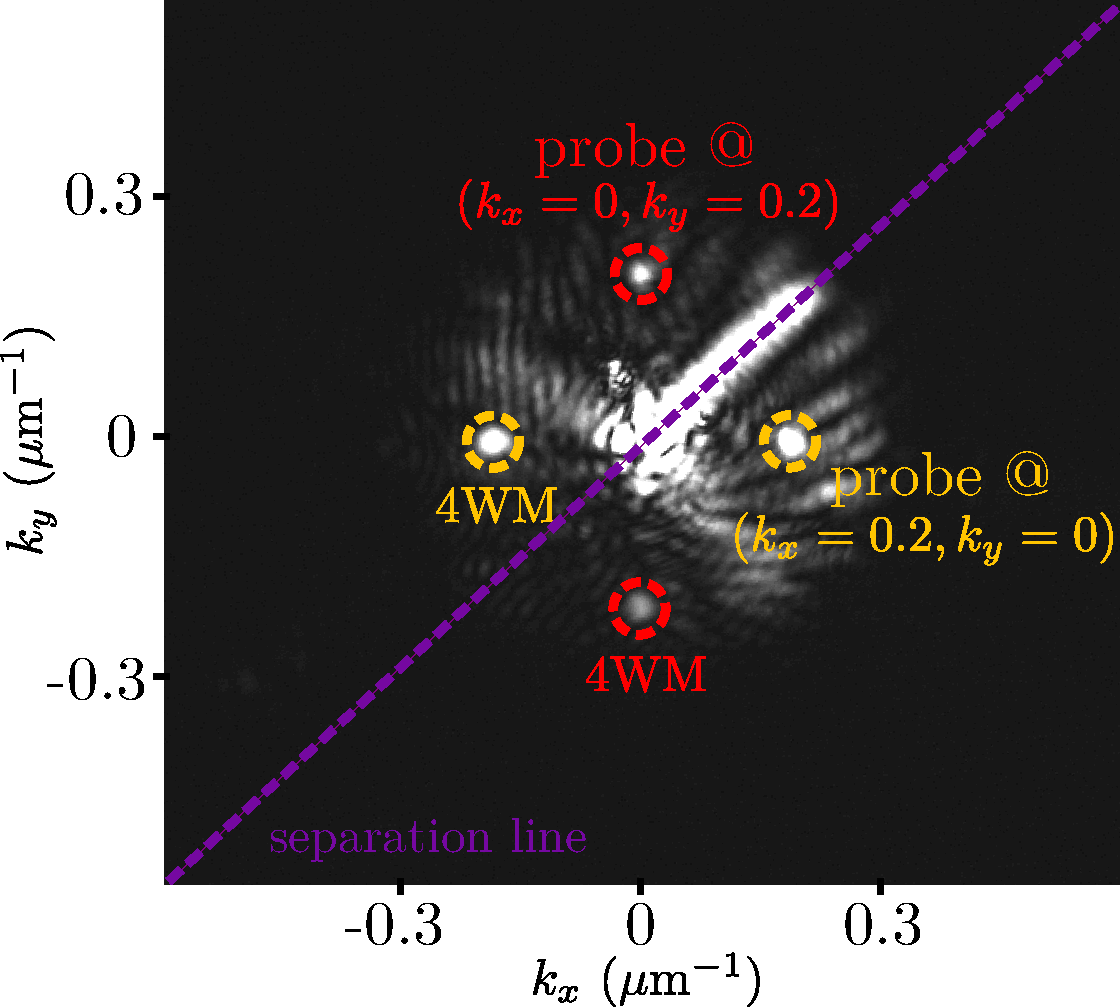
\includegraphics[width=1\textwidth]{chap_correlation/fig/mosaic_4wm.pdf}
    \caption{\textbf{Fourier plane of the field with two probe beams injected in the system}. The two beams are injected at $k_{pr}=(0.2,0)$ and $k_{pr}=(0,0.2)$. The red dashed circle represent the conjugate mode along the $y$-axis and the yellow dashed circles the modes along the $x$-direction. The half mirror is rotated by 45° to separate the top left and right bottom part of the field
    which is represented by the purple dashed line. The pinholes are placed in the Fourier plane at the appropriate wavevector to measure the correlations between two conjugate modes or between two modes that are not conjugate.}
    \label{fig:sanity_check}
\end{figure}

\bigskip

\indent \textbf{Experiment check.} To validate that the apparatus is able to measure correlations between the Bogoliubov modes and is not only measuring the single mode character of the polariton fluid \cite{a_baas_quantum_degeneracy2006}, we inject two probe beams in the system in order to generate two independent 
four wave mixing processes. Both of them come from the same laser : one has a non zero wavevector along the $x$-axis $(k_x=0.2, k_y=0)$ while the other one has a non zero wavevector along the $y$-axis $(k_x=0, k_y=0.2)$. For the sake of clarity we label $k_{x,y}$ the modes directly excited by the probe and $k_{x,y}^*$ their conjugate counterpart. The energy of the laser is again set to be resonant with the normal branch of the Bogoliubov dispersion.
Each of the two probe beams generates its own conjugate mode at its respective opposite wavevector as shown in \autoref{fig:sanity_check}. 
One can notice that the modes along the $y$-axis are less intense than these along $x$ despite the input size and intensity of the two beam is the same. This once again supports the idea that the emission efficiency in one mode or the other is $k$-dependent. 

The verification consists in measuring the correlations between two conjugate modes and compare it to the correlation between two modes that are independent.
If the measurement is dominated by pump contributions one should measure the same result for both cases. To do so, we rotate the half mirror by 45° around its normal axis in order to separate the top left part of the field from the bottom right part and send them to the two optical paths. The separation is explicited
by the diagonal purple dashed line in \autoref{fig:sanity_check}. Then, depending on which couple we want to measure the correlations, we place the pinholes in the Fourier plane at the appropriate wavevector.
The results are shown in \autoref{fig:noise_comparison}. The panel \textbf{a)} displays the PSD of the photocurrent difference for the two conjugate modes $k_x$ and $k_x^*$ while \textbf{b)} shows the same measurement for the two modes $k_y$ and $k_y^*$. 
A simple way to infer if the beams are correlated is to compare the difference PSD to the sum of the individual PSDs. From \autoref{eq:diff_psd2} on can see that these two quantities are equal in the absence of correlation ie when $C=0$. As visible, in the first case \textbf{a)}, the difference PSD is below the sum of the individual PSDs, which indicates that the two modes are correlated. In contrast, in the second case \textbf{b)}, the difference PSD is superimposed to the sum of the individual PSDs, which indicates that the two modes are not correlated. 

More precisely, we measure a correlation coefficient $C_{k_x,k_x^*}=0.11\pm{0.01}$ for the first case and $C_{k_x,k_y^*}=0.01\pm{0.005}$ for the second one. The error bars are estimated from the standard deviation of the PSDs over the swipe time of the spectrum analyzer.
This result confirms that modes originating from the same four wave mixing process are correlated while modes originating from different processes are not and that the measurement is 
not dominated mean field contributions.


\begin{figure}
    \centering
    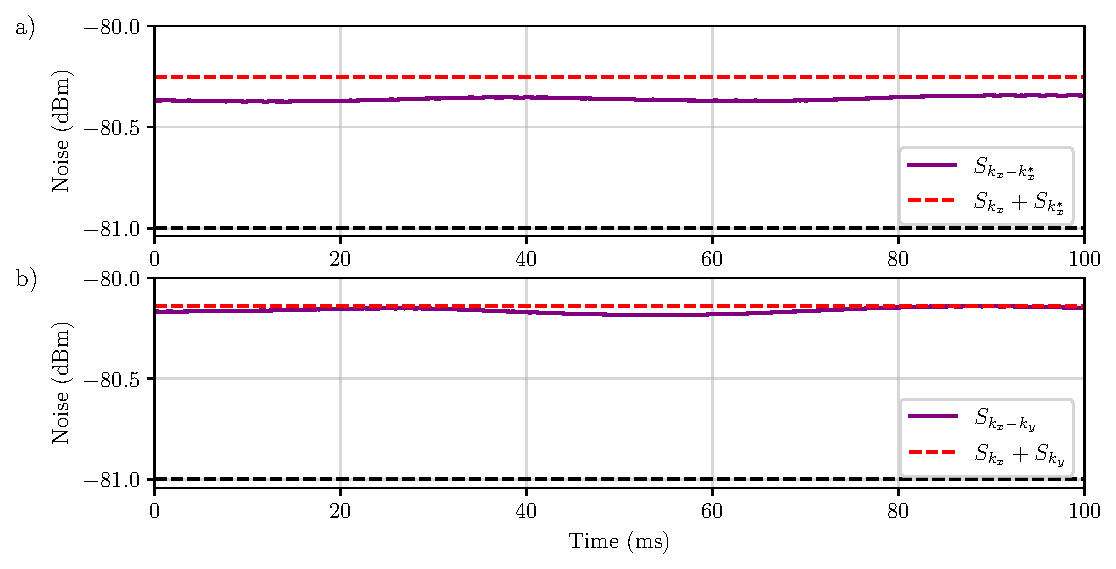
\includegraphics[width=1\textwidth]{chap_correlation/fig/noise_comparison.pdf}
    \caption{Sanity check correlation measurement. \textbf{a)} Power spectral density of the photocurrent difference for two conjugate modes $k_x$ and $k_x*$. \textbf{b)} Power spectral density of the photocurrent difference for two modes that are not conjuated $k_x$ and $k_y^*$. To smooth 
    the data, the noise is averaged on 10 sweeps of the spectrum analyzer. In both panels, the red dashed line represents the sum of the two individual photocurrent PSD measured independently. The black dashed line is the dark electronic noise of the apparatus.} 
    \label{fig:noise_comparison}
\end{figure}



\subsubsection{Correlations measurement}
\label{sec:exp_corr_measurement}

The previous section showed that the efficiency of the emission in a given mode appears to be $k$-dependent. As a consequence, studying correlations for different probe wavevectors might not be the best way to investigate the Bogoliubov modes correlations.
Instead, we propose to focus on the correlations as a function of the operating point of the polariton fluid on the higher branch of the bistability loop. 

To do so, we fix the probe wavevector to $k_{pr}=(0\ ,\ \SI{0.2}{\per\micro\meter})$ and set the pump intensity to operate on the high density branch of the hysteresis curve. Then the pump power is ramped down toward the turning point of the bistability loop.
In terms of collective excitation, the system goes from a parabolic gapped dispersion to a linear gapless one as explained in \autoref{chap:generation_transonic_fluid}.


\begin{figure}
    \centering
    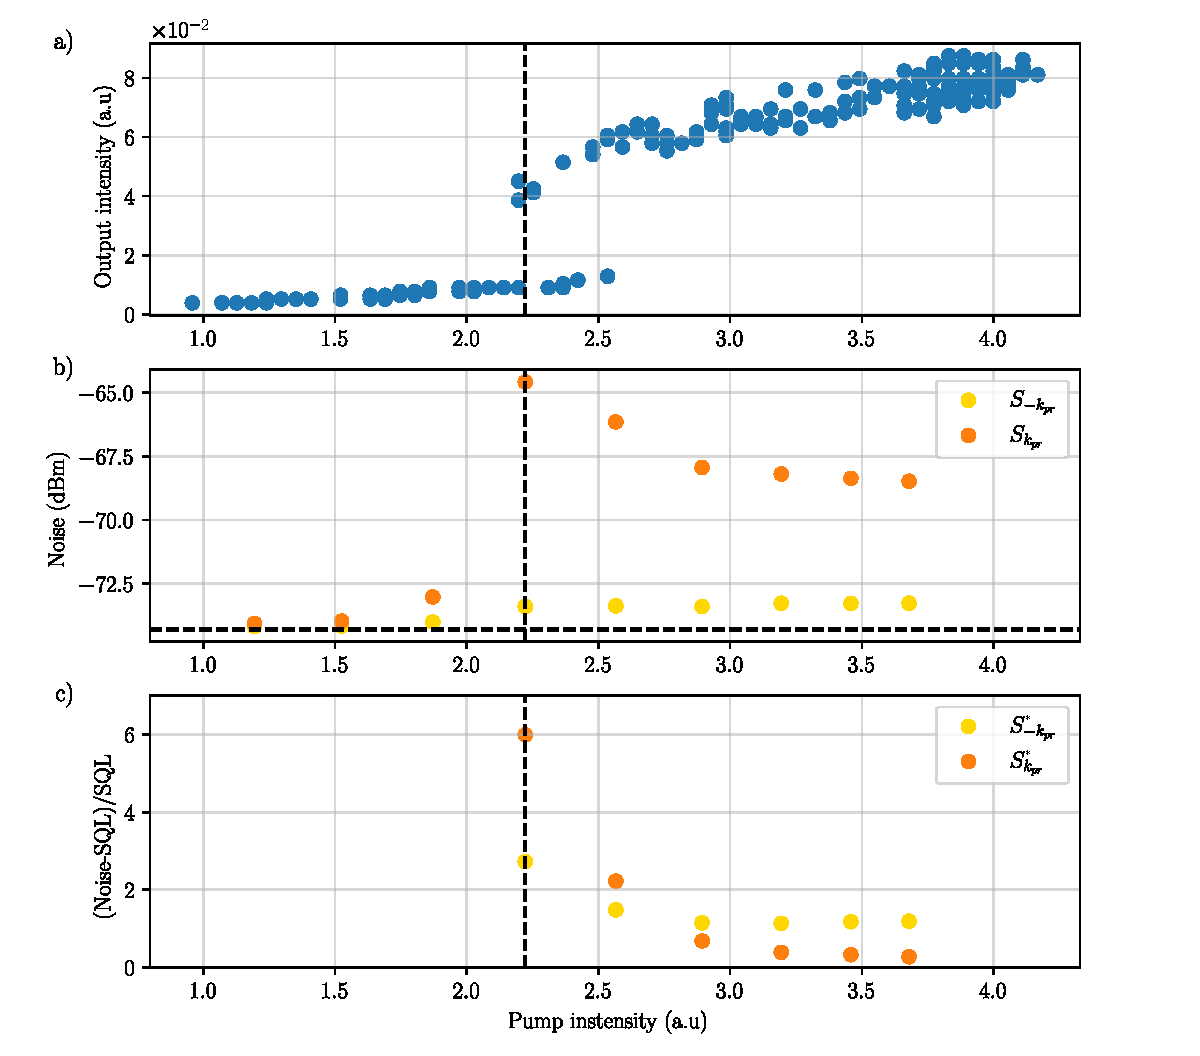
\includegraphics[width=1\textwidth]{chap_correlation/fig/noises_vs_bistab.pdf}
    \caption{\textbf{a)} Measured bistability loop of the static polariton fluid at the working point B10-C10 with detuning $\delta=\SI{35}{\giga\hertz}$. The vertical black dashed line on all plots
    indicates the turning point of the bistability loop. \textbf{b)} Measurement of the individual noises of the two conjugate modes $k_{pr}$ and $-k_{pr}$ as a function of the pump power. The horizontal black dashed line represent the dark noise of the apparatus.
    \textbf{c)} Excess noises of the two conjugate modes normalized to their respective shot noise calculated from the calibration curve of \autoref{fig:calibration}. The points at pump power below the turning point are not shown because they were to weak to be measured and fall in the dark noise of the apparatus.}
    \label{fig:noises_vs_bistab}
\end{figure}


At each pump power, the probe frequency is tuned to stay resonant with the normal branch Bogoliubov mode at $k_{pr}$. The correlations between the two conjuate mode are then measured the same way as in the previous section. 
We start by analyzing the noise of each mode based on \autoref{fig:noises_vs_bistab}. The first plot in \autoref{fig:noises_vs_bistab}~\textbf{a)} shows the bistability loop of the polariton fluid under investigation. 
The measurement of the individual noises is displayed in \autoref{fig:noises_vs_bistab}~\textbf{b)}. The normal branch mode is much more noisy than its conjugate counterpart. This is mainly due to the power unbalance between the two modes. To compare them 
on the same scale we normalize their excess noise to their respective shot noise calculated from the calibration curve of \autoref{fig:calibration} and plot the result in \autoref{fig:noises_vs_bistab}~\textbf{c)}. The normalized excess noise are labelled $S_{k_{pr},-k_{pr}}^*$ for the sake of clarity. Both exhibit excess noise due to nonlinear interactions \cite{a_baas_quantum_degeneracy2006}. Then the noises increase significantly when the system
approaches the turning point. This is a typical feature of critical points and phase transitions in physical systems. For example, such behavior is closely analogous to what occurs in an optical parametric oscillator (OPO) configuration just below threshold
\cite{Zhang:06} : the amplitude quadrature of the signal and idler drastically increase in a correlated way
leading to the formation of two modes squeezed state. 

\bigskip


In a second time we measure the noise of the difference photocurrent and compute the corresponding correlation in \autoref{fig:c_vs_bistab}. In order to easily see the evolution of the correlations, we also plot the sum of the individual noises as if they were not correlated like we did previously. When the system is far from the turning point and is not even bistable, the difference PSD is almost superimposed to the sum of the individual PSDs which, as shown in \autoref{fig:c_vs_bistab}. This behavior indicates a low correlation between the two modes ($C_{k_{pr},-k_{pr}}\approx0.02$).
When the system gets closer to the turning point, the difference PSD becomes lower than the sum of the individual PSDs and the correlation increases to reach a maximum value of $C_{k_{pr},-k_{pr}}=0.61\pm0.05$ near the turning point. It is likely that the correlations would further increase if we were able to operate even closer to the turning point. However, this is not possible in practice because at this point the system becomes
unstable and any fluctuation makes the system fall back to the low density branch of the bistability loop.

Furthermore, if we refer 
to the ideal linear amplifier model \cite{boyd_nl_optics}, increasing the amount of nonlinearity in order to increase the gain of the four wave mixing process should in principle enhance the correlations as well. In a polariton
system, this can be achieved by increasing the detuning $\delta$ between the pump laser and the polariton resonance. However, this implies high pump laser power to remain in the bistable regime and, up to a certain point, the laser starts to heat the sample which in turn results in a reduction of the nonlinearity and thus of the correlations \cite{romanelli_4wm_2007}.


Finally, one might consider that balancing the signals by attenuating the mode on the normal branch could enhance the observed correlations.
 In fact the work \cite{Romanelli:04} showed that rather than balancing the beam intensities, correlations could 
be enhanced by balancing the individual noises of the two modes. However, in our case the two intensities and two individiual noises differ by a factor 10 and 7 respectively. In any case, such attenuation introduces excessive losses on the normal branch mode and causes its intensity statistics to approach a Poissonian distribution, thereby suppressing the correlations.
In any case, such attenuation introduces excessive losses on the normal branch mode and causes its intensity statistics to approach a Poissonian distribution, thereby suppressing the correlations.





\begin{figure}
    \centering
    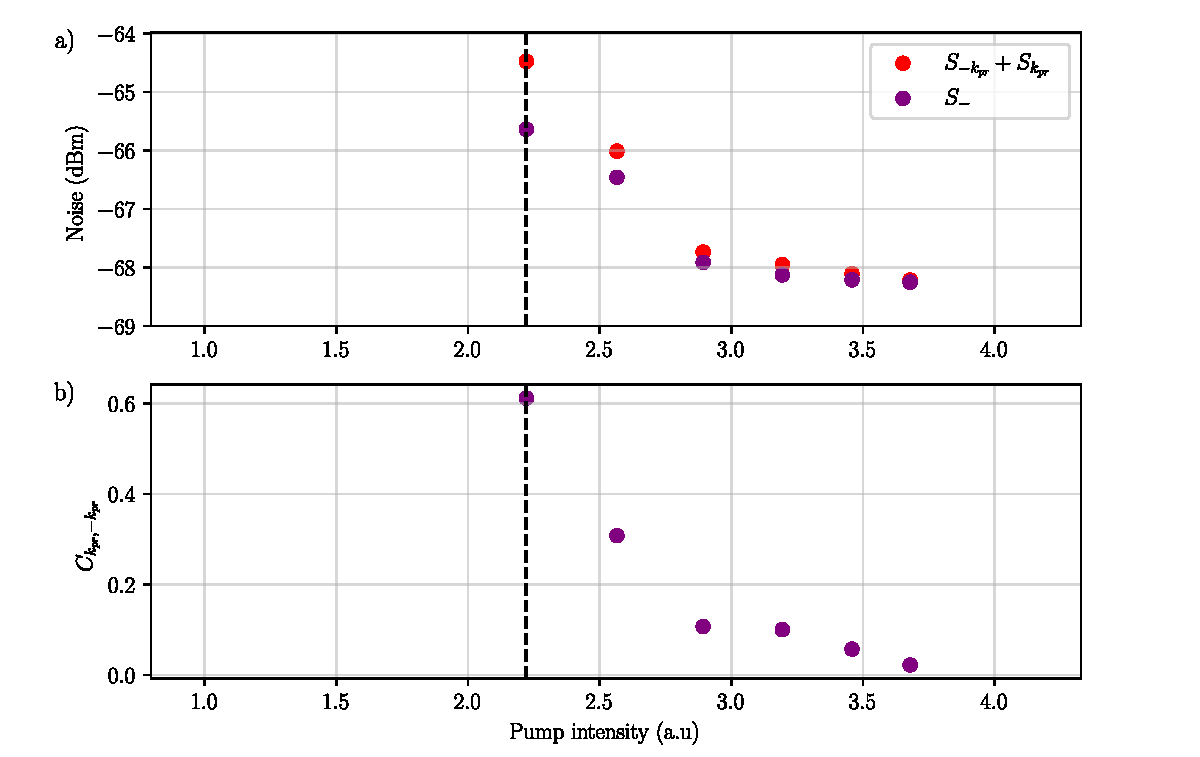
\includegraphics[width=1\textwidth]{chap_correlation/fig/correlation_vs_bistab.pdf}
    \caption{Correlations between Bogoliubov modes as a function of the pump power. 
    \textbf{a)} Measurement of the difference photocurrent noise. The latter is represented by the purple dots while the red dots indicates the sum of the individual noises measured independently. \textbf{b)} Correlation coefficient $C_{k_{pr},-k_{pr}}$ between the two conjugate modes as a function of the pump power.}
    \label{fig:c_vs_bistab}
\end{figure}


\section{Conclusion}

In this chapter, we have investigated the correlations between Bogoliubov modes in a polariton quantum fluid. By employing a balanced detection scheme, we were able to measure the intensity correlations between the normal and ghost branches of the Bogoliubov dispersion. The experimental results demonstrate that these correlations are seeded by the nonlinear four-wave mixing process intrinsic to the polariton system.

We first validated the experimental setup by ensuring that the lasers used in the experiment were shot-noise limited and that the balanced detection scheme was capable of isolating quantum correlations from classical noise. An experiment check confirmed that the measured correlations were indeed due to the nonlinear scattering process and not dominated by residual pump contributions or single-mode effects.

The analysis of the Bogoliubov coefficients revealed that the emission in the normal and ghost branches becomes balanced at low wavevectors, despite showing an asymmetry suggesting a $k$-depence in the emission efficiency. Furthermore, we observed that the correlations increase significantly as the system approaches the turning point of the bistability loop, where the four-wave mixing process is the most efficient. This behavior highlights the critical role of the bistable regime in amplifying quantum correlations.

The maximum correlation coefficient measured was $C_{k_{pr},-k_{pr}} = 0.61 \pm 0.05$, achieved near the turning point of the bistability loop. This result demonstrates the potential of polariton systems for generating strongly correlated quantum states, which could be further optimized by operating closer to the turning point or by tuning the system parameters to enhance the nonlinear gain.

